\chapter{Rastreabilidade}

Nesta seção, será abordada a matriz de rastreabilidade envolvendo os requisitos elicitados.

\subsection{Rastreabilidade Vertical}
Segundo Dall'Oglio, a rastreabilidade vertical está relacionada com a capacidade de detectar relacionamento entre artefatos dependentes dentro de um modelo de processo utilizado. Neste trabalho, essa rastreabilidade se dá entre os Épicos, Features e Histórias de Usuário, a ferramenta TargetProcess foi utilizada para cadastro desses requisitos, a mesma também disponibiliza um sistema de rastreabilidade, sendo exemplificada nas figuras abaixo.


\begin{figure}[!htpb]
\centering
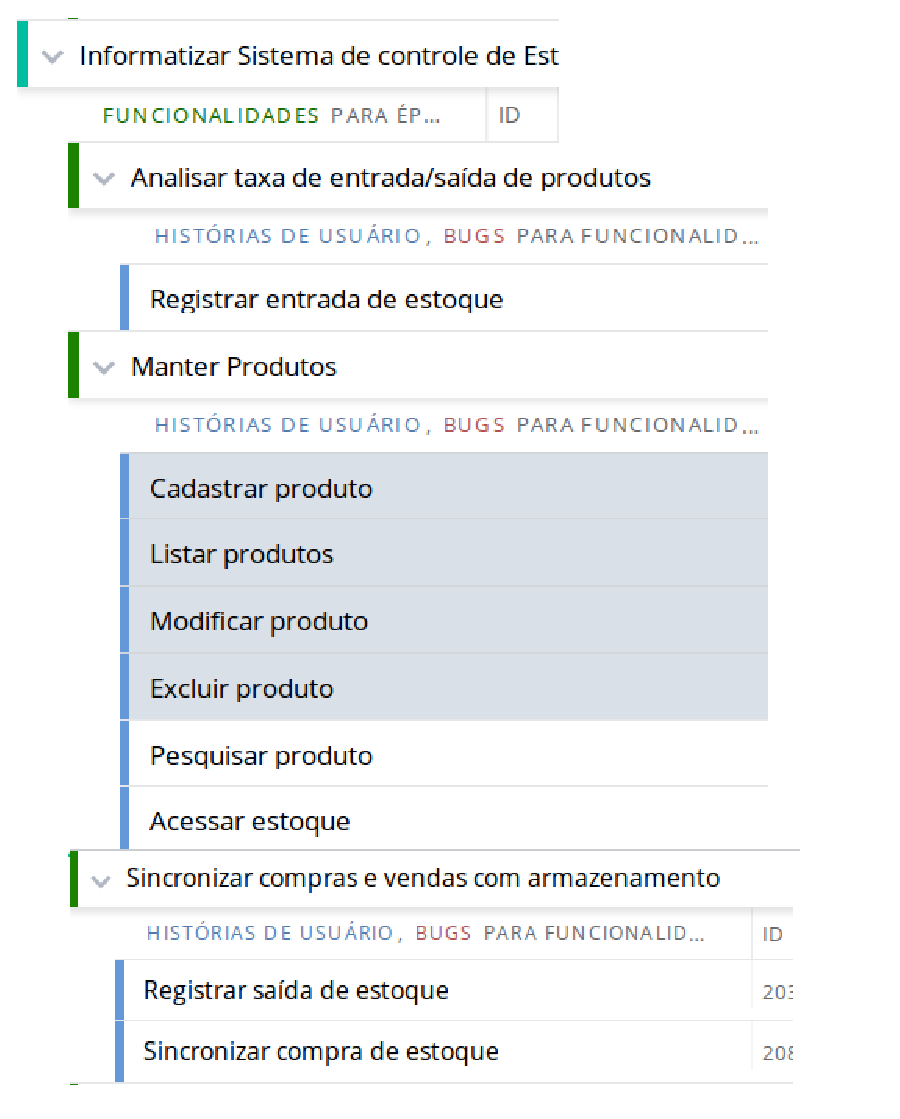
\includegraphics[scale=0.4]{figuras/processo/epico1}
\caption{Rastreabilidade vertical do EP01.}
\end{figure}


\begin{figure}[!htpb]
\centering
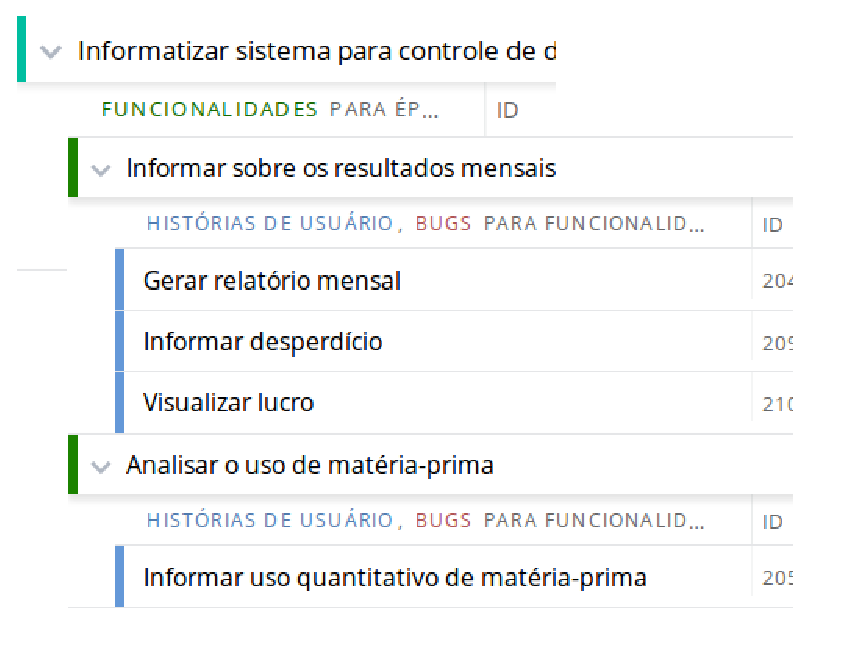
\includegraphics[scale=0.35]{figuras/processo/epico2}
\caption{Rastreabilidade vertical do EP02.}
\end{figure}

\subsection{Rastreabilidade Horizontal}
Segundo Dall'Oglio, essa rastreabilidade está relacionada com a habilidade de relacionar artefatos entre diferentes modelos, dentre esses artefatos podem estar requisitos, artefatos de análise, de design, entre outros. Seguem exemplos dessa rastreabilidade aplicado no trabalho logo abaixo:

\begin{figure}[!htpb]
\centering
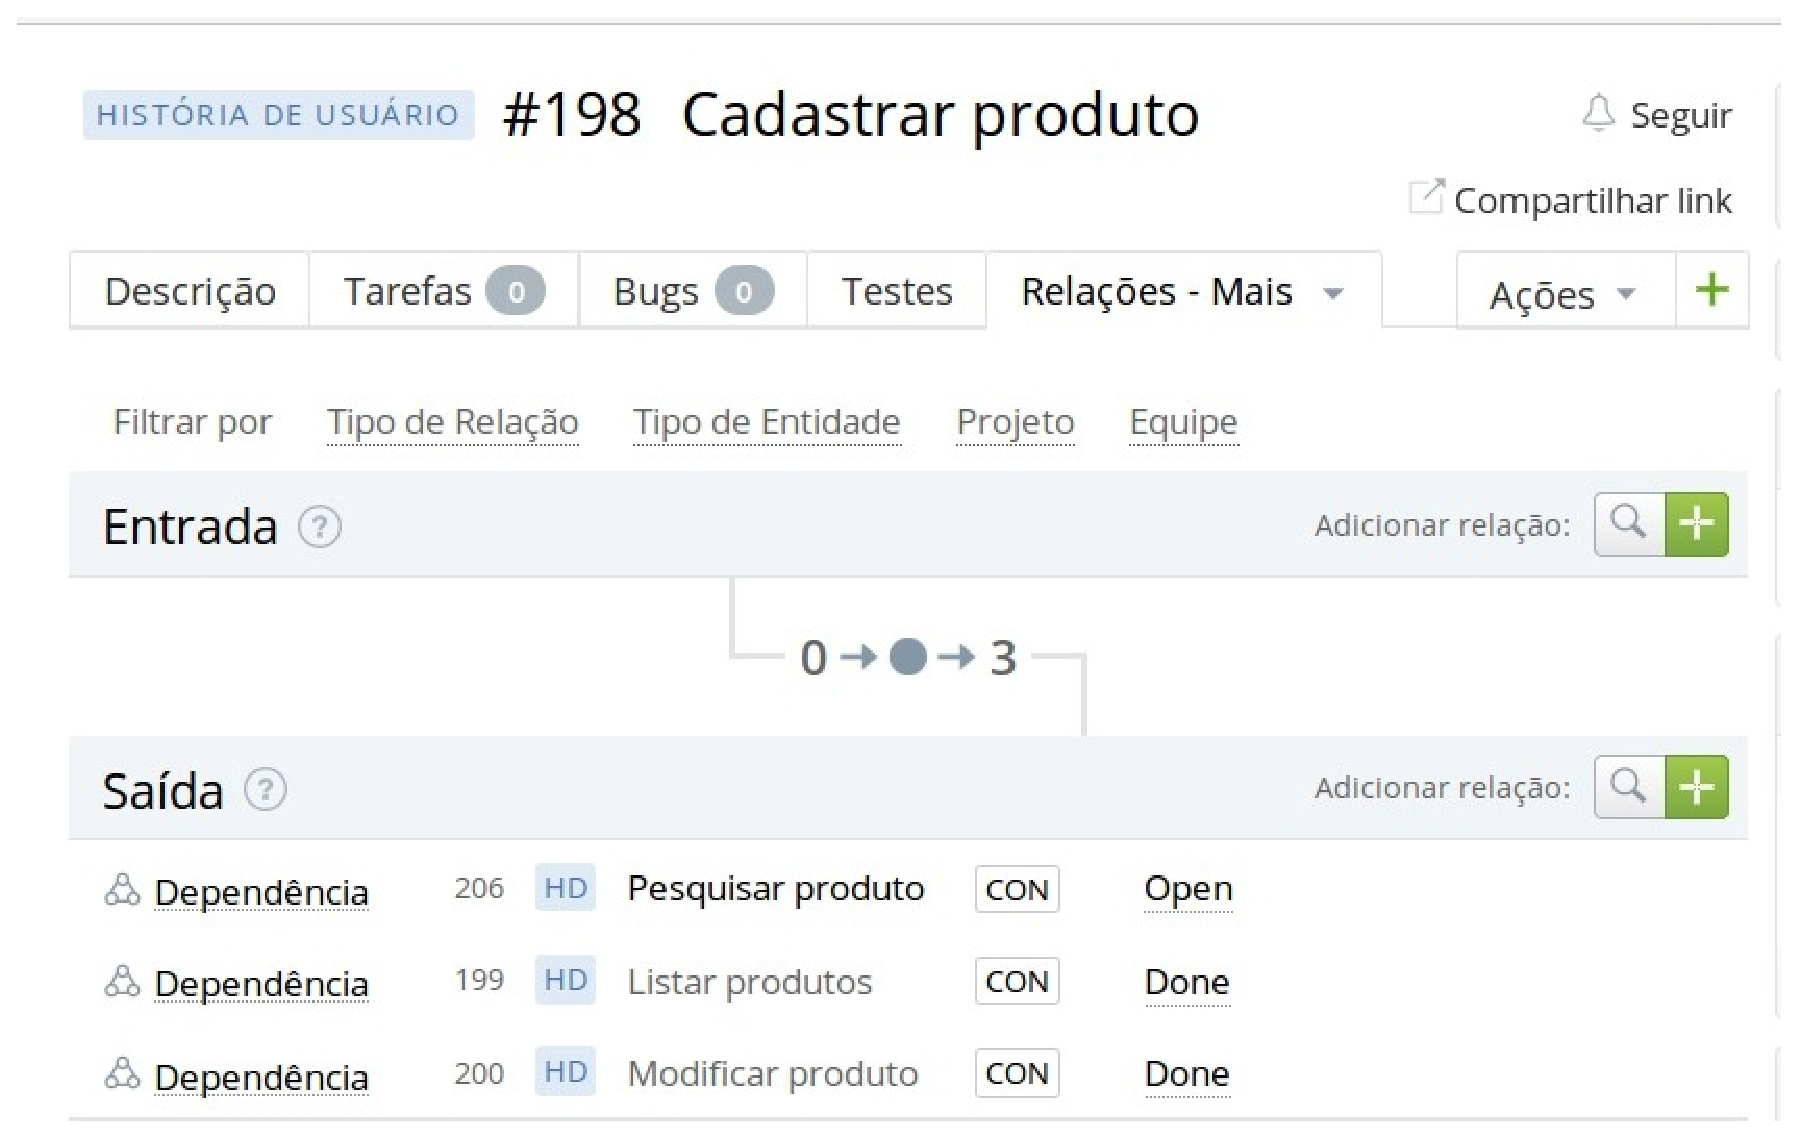
\includegraphics[scale=0.6]{figuras/gerenciamento/foto}
\caption{Pesquisar produto, Listar produto, Modificar produto são dependentes da história Cadastrar Produto.}
\end{figure}